کد پیوست‌شده ۲۰ بار بازی را با توزیع‌های فرکانس اولیه مختلف اجرا می‌کند. هر بار که بازی اجرا می‌شود، فرکانس‌های استراتژی‌ها را در پایان بازی نمایش می‌دهد.

با توجه به نتایج نمودارها، می‌توانیم ببینیم که چه نوع توزیع‌های پایداری وجود دارد.

برای بررسی چگونگی رسیدن به حالات پایدار، باید به چگونگی تغییر فرکانس‌ها در طول زمان توجه کنیم. اگر فرکانس‌های استراتژی‌ها به طور کلی به سمت حالت پایدار تغییر می‌کنند، این نشان می‌دهد که حالت پایدار یک جاذبه است. در غیر این صورت، باید بررسی کنیم که چه عواملی باعث ایجاد حالت پایدار شده‌اند. برای مثال، اگر یک استراتژی در ابتدا فرکانس بالایی دارد، این ممکن است باعث شود که این استراتژی به حالت پایدار تبدیل شود.

بازی تقسیم کیک یک بازی است که در آن هر بازیکن یک تقاضا (استراتژی) از 0 تا 10 اعلام می‌کند. اگر مجموع تقاضاها بیش از 10 باشد، هر دو بازیکن صفر دریافت می‌کنند. در غیر این صورت، هر بازیکن تقاضای خود را به عنوان پاداش دریافت می‌کند.

در شبیه‌سازی بازی با استفاده از پویایی تکثیرگر 
\lr{(Replicator Dynamics)}
، هر بازیکن به صورت تصادفی یک بازیکن دیگر را انتخاب می‌کند و اگر پاداش آن بازیکن بیشتر باشد، استراتژی آن بازیکن را اتخاذ می‌کند. در نتیجه، استراتژی‌هایی که پاداش بیشتری را ارائه می‌دهند، به مرور زمان بیشتر منتشر می‌شوند.

حالت‌های پایدار در این بازی حالت‌هایی هستند که بعد از رسیدن به آن‌ها، فرکانس استراتژی‌ها تغییر نمی‌کند. این حالت‌ها می‌توانند به دو دسته کلی تقسیم شوند:

حالت‌های پایدار سطحی 
\lr{(Surface Equilibria)}
: در این حالت‌ها، بعضی از استراتژی‌ها فرکانس ثابتی دارند و بقیه به صفر می‌رسند. برای مثال، اگر تمام بازیکنان تقاضای 5 داشته باشند و هیچ کس تقاضای بیشتری نداشته باشد، بازی به یک حالت پایدار سطحی می‌رسد.

حالت‌های پایدار نقطه‌ای 
\lr{(Point Equilibria)}
: در این حالت‌ها، فقط یک استراتژی فرکانس مثبت دارد و بقیه به صفر می‌رسند. برای مثال، اگر تمام بازیکنان تقاضای 10 داشته باشند، بازی به یک حالت پایدار نقطه‌ای می‌رسد.

در بررسی حالت‌های پایدار مختلف، باید توجه کرد که حالت پایدار نهایی به توزیع اولیه فرکانس‌ها بستگی دارد. به عنوان مثال، اگر فرکانس اولیه استراتژی‌های بالاتر بیشتر باشد، احتمال رسیدن به حالت پایدار با فرکانس بالایی برای این استراتژی‌ها بیشتر است. از طرفی، اگر فرکانس اولیه استراتژی‌های پایین‌تر بیشتر باشد، احتمال رسیدن به حالت پایدار با فرکانس بالایی برای این استراتژی‌ها بیشتر است.

برای درک بهتر حالت‌های پایدار، می‌توان با استفاده از شبیه‌سازی و با تغییر دادن توزیع فرکانس اولیه، مشاهده کرد که چگونه به حالت‌های پایدار مختلف می‌رسیم.

حالا نمودارهای داخل کد را تحلیل می‌کنیم:

در این تصاویر، نمودار ستونی میزان استفاده کل جامعه از استراتژی‌ها را بیان می‌کند و قسمت افقی بیانگر گذشت نوبت‌هاست. 

حالا ما ۲۰ تا تصویر داریم ولی به مقایسه‌ی برخی از آن‌ها و بررسی روند پیشرفت هر کدام از استراتژی‌ها می‌پردازیم.

\begin{center}
	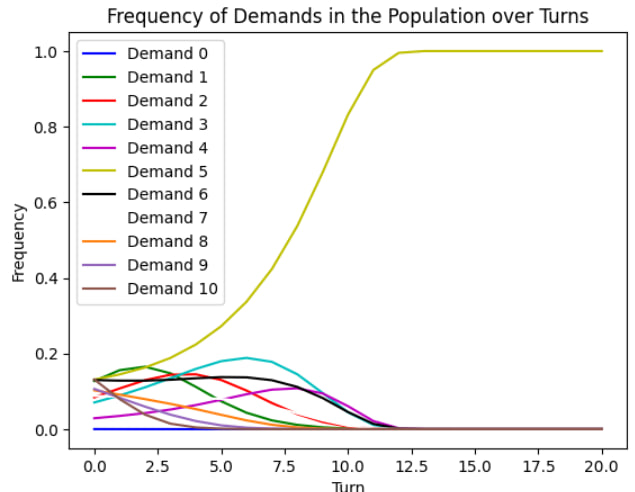
\includegraphics{1}
\end{center}

در این تصویر، در ابتدا استراتژی درخواست ۱، ۳، ۵ کمی رشد می‌کنند اما مابقی کاهش میابند. این امر واضح هست زیرا در تمام حالات دیگر یا پاداش کم بوده و یا انقدر خواسته زیاد است که با هیچ بازیکن دیگر سازگار نمی‌شوند. بعد از مدتی فقط استراتژی ۵ در حال رشد کردن است، زیرا که اکثر بازیکنان یا درحال بازی چهار استراتژی ۳، ۴، ۵ و ۶ هستند و پس از ۱۲ نوبت تقریبا همه‌ی بازیکنان استراتژی ۵ را به عنوان استراتژی خود انتخاب می‌کنند.

مهم اینجا این است که استراتژی انتخابی بازیکنان به طور کامل وابسته به استراتژی جامعه است. اگر مقادیر اولیه متفاوتی داشته باشیم، به استراتژی‌های مختلفی همگرا می‌شویم. این استراتژی‌ها عموماً محدود به فقط ۵، یا ۴ و ۶ یا ترکیبی از آنها هستند. در برخی از نمودارها، با شیب بیشتری به سمت استراتژی پایدار همگرا می‌شویم، در حالی که در بخش‌های دیگر این شیب کمتر است، که در ادامه به آن خواهیم پرداخت.

\begin{center}
	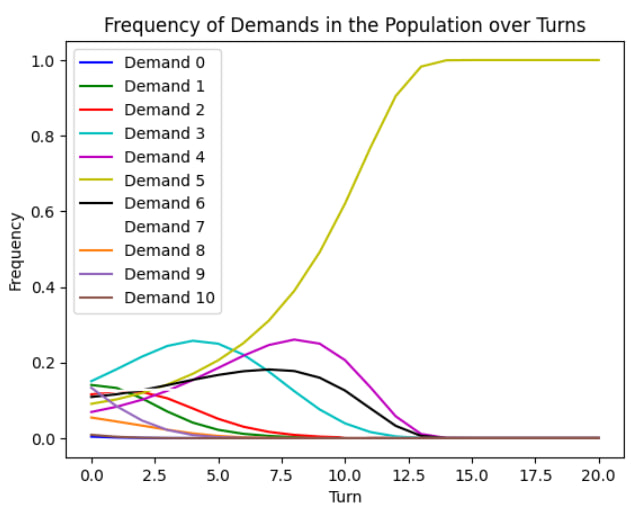
\includegraphics{2}
\end{center}

این‌جا نیز مشابه حالت قبل رخ می‌دهد و نکته این است که پس از ۱۳ نوبت تقریبا همه‌ی بازیکنان استراتژی ۵ را به عنوان استراتژی خود انتخاب می‌کنند.

\begin{center}
	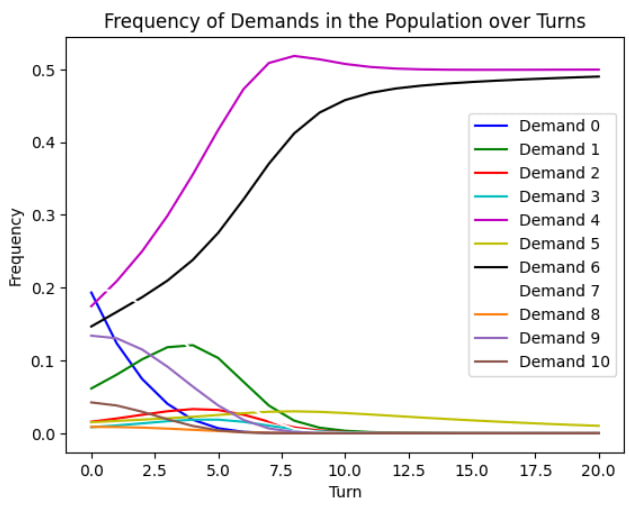
\includegraphics{3}
\end{center}

اما در این نمودار، در ابتدا استراتژی‌های ۱، ۹، ۴ و ۶ در حال رشد هستند و نکته این است که تا وقتی کسانی داریم که استراتژی ۹ انتخاب می‌کنند، افرادی هم هستند که استراتژی مکمل آن را انتخاب کنند و ۱ انتخاب شود تا خواسته‌ی سوال برآورده شود و در نتیجه این دو موازی هم پیش می‌روند ولی در نهایت پس از حد ۹ ام، اکثر بازیکنان استراتژی ۴ و ۶ را انتخاب می‌کنند؛ اما استراتژی ۵ نیز کمی بازی می‌شود و بازیکنانی هستند که ۵ را انتخاب کنند تا آخرِ حرکت ۲۰ ام.

\begin{center}
	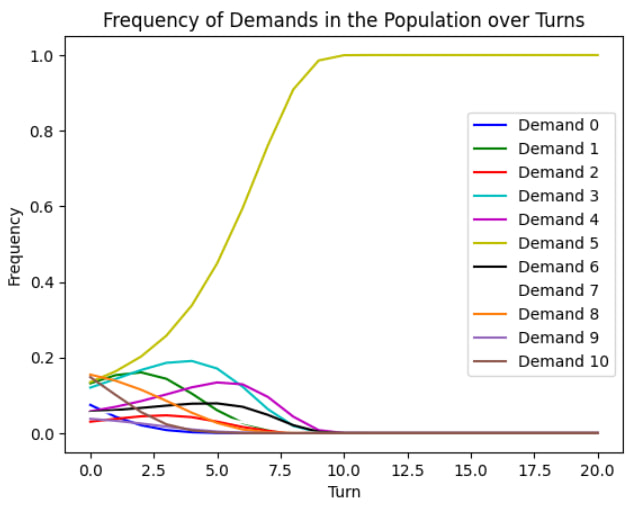
\includegraphics{4}
\end{center}

\begin{center}
	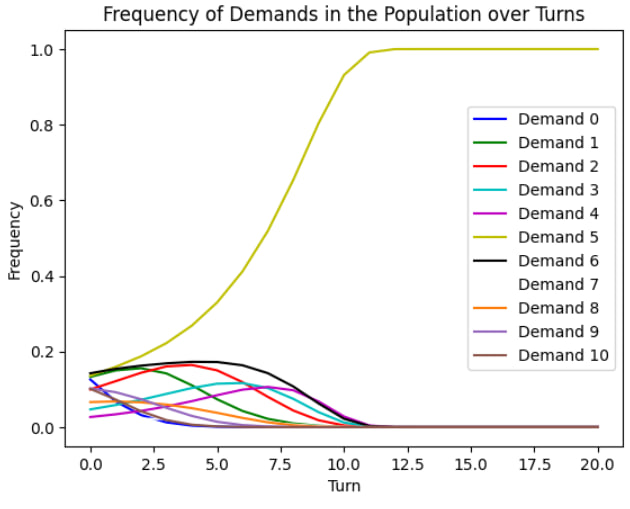
\includegraphics{5}
\end{center}

\begin{center}
	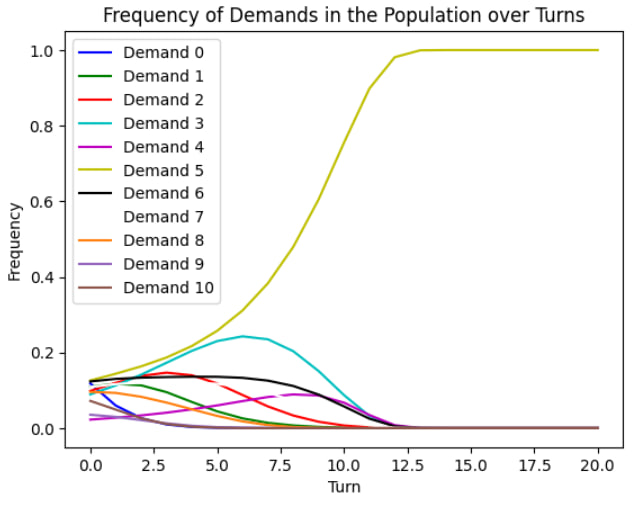
\includegraphics{6}
\end{center}

\begin{center}
	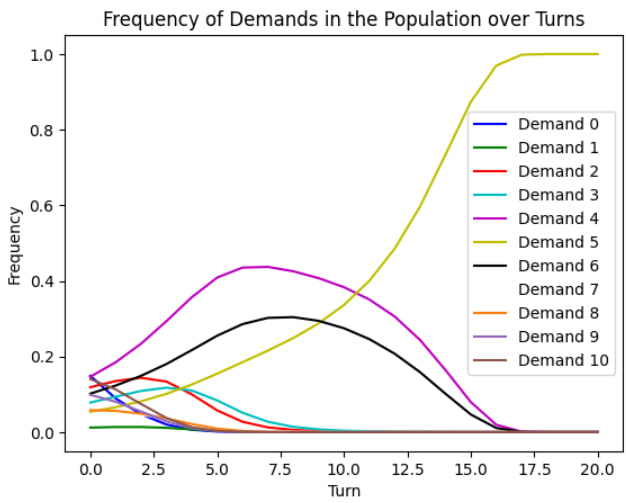
\includegraphics{7}
\end{center}

همه‌ی نمودارهای بالا در این بخش، در نهایت اما با شیب‌های متفاوت، به استراتژی ۵ میل می‌کنند و هر کدام مسیر متفاوتی دارند تا پایداری.

\begin{center}
	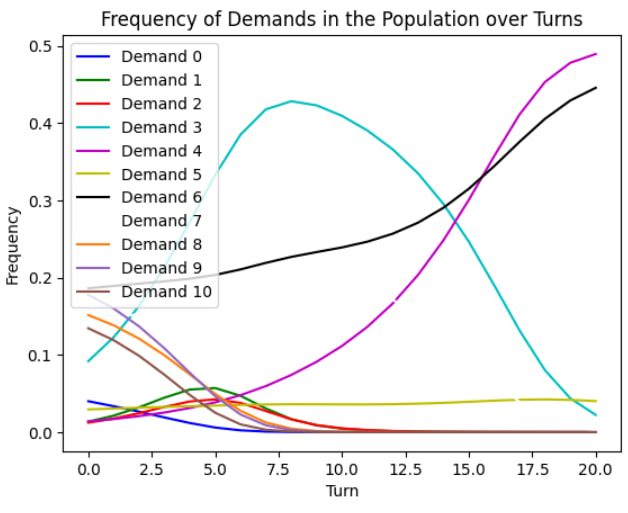
\includegraphics{8}
\end{center}

این نمودار اما خیلی نکته‌دار است. در این نمودار، استراتژی‌های ۳، ۷، ۴، ۶ و ۵ به طور کلی در حال رشد هستند و به‌مرور به ۴ و ۶ پایدار می‌شوند در حرکات نهایی و باقی استراتژی‌ها کم‌رنگ‌تر می‌شوند.

همان‌طور که بالاتر گفتیم،
وقتی کسانی داریم که یک استراتژی انتخاب می‌کنند، افرادی هم هستند که استراتژی مکمل آن را انتخاب کنند و در نتیجه تشکیل نمودارها بدین شکل است.

در ادامه باقی تصاویر بدست آمده را در این‌جا قرار می‌دهیم و نتیجه‌گیری می‌کنیم از شکل نمودارها به طور کلی.

\begin{center}
	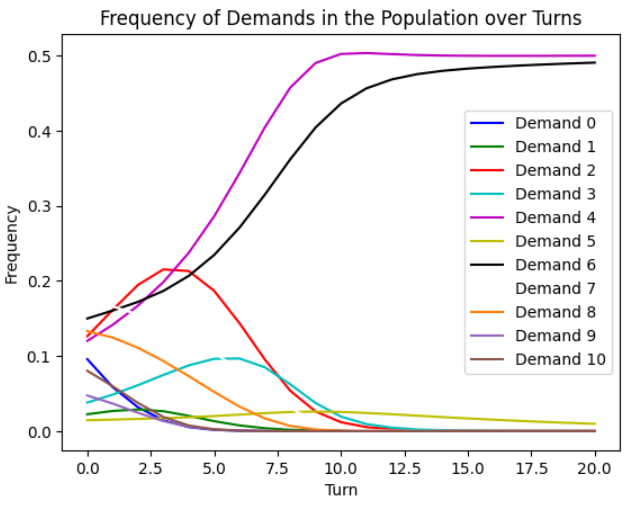
\includegraphics{9}
\end{center}

\begin{center}
	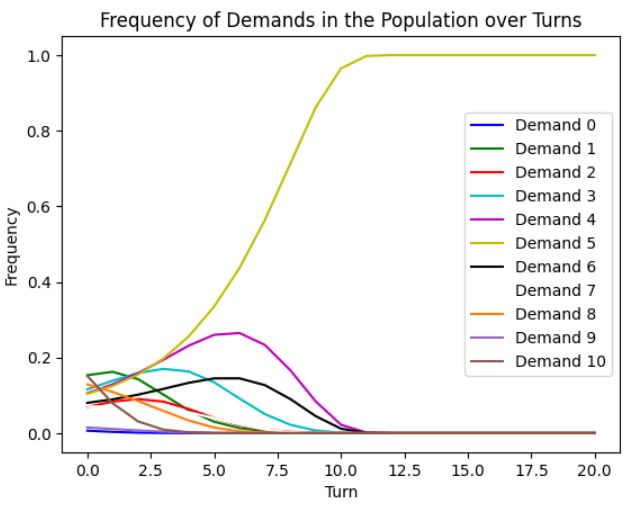
\includegraphics{10}
\end{center}

\begin{center}
	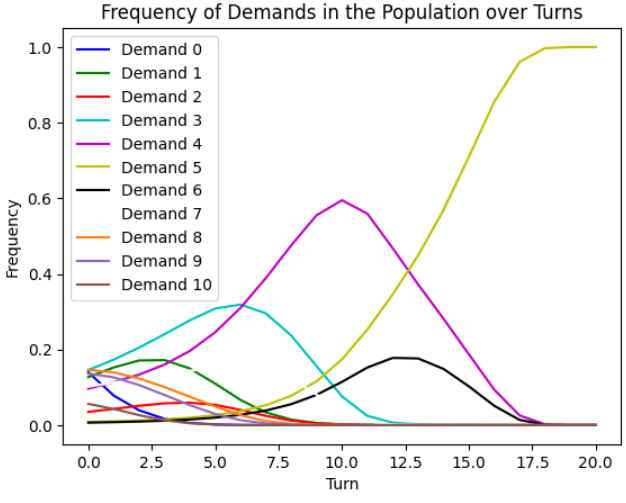
\includegraphics{11}
\end{center}

\begin{center}
	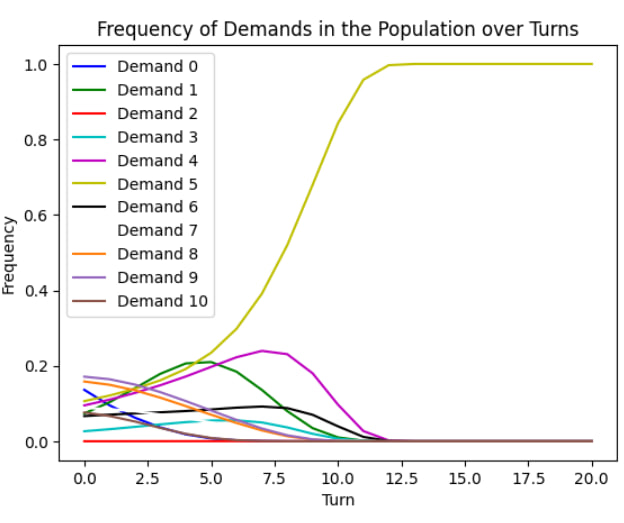
\includegraphics{12}
\end{center}

\begin{center}
	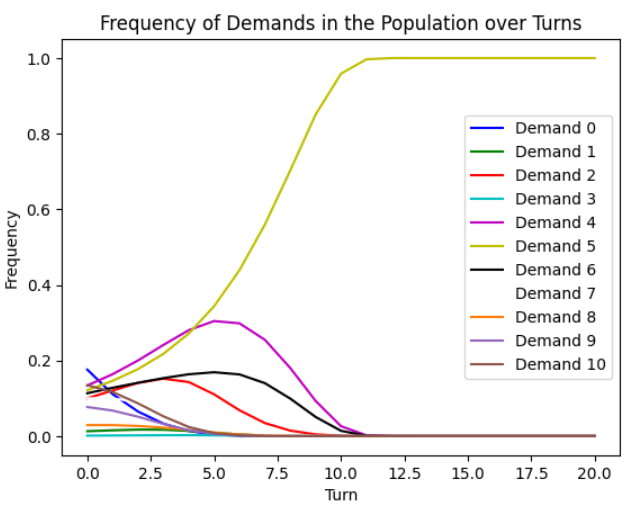
\includegraphics{13}
\end{center}

\begin{center}
	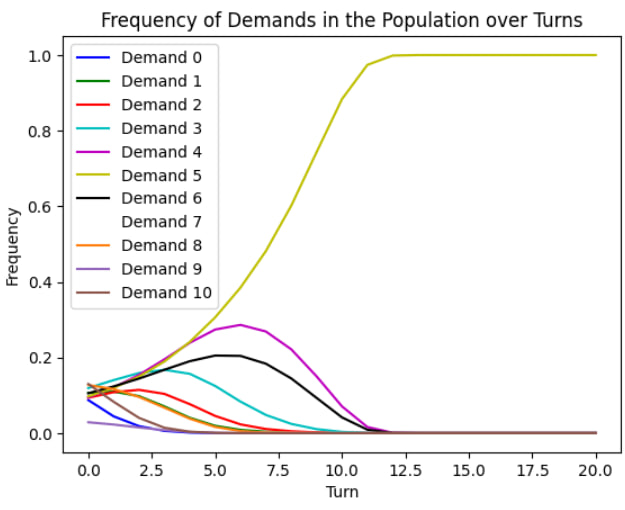
\includegraphics{14}
\end{center}

\begin{center}
	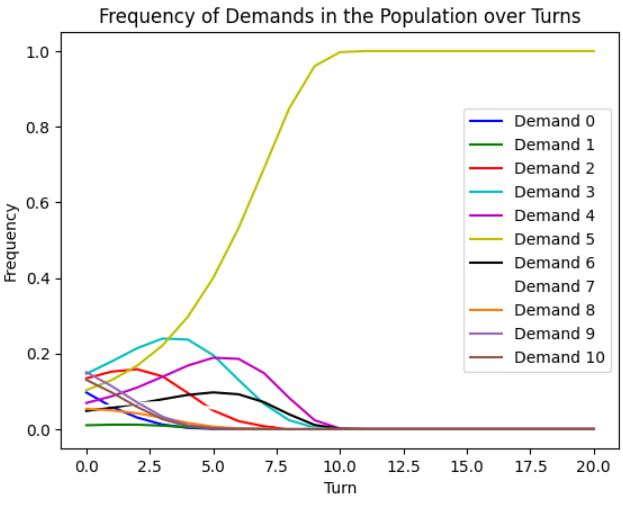
\includegraphics{15}
\end{center}

\begin{center}
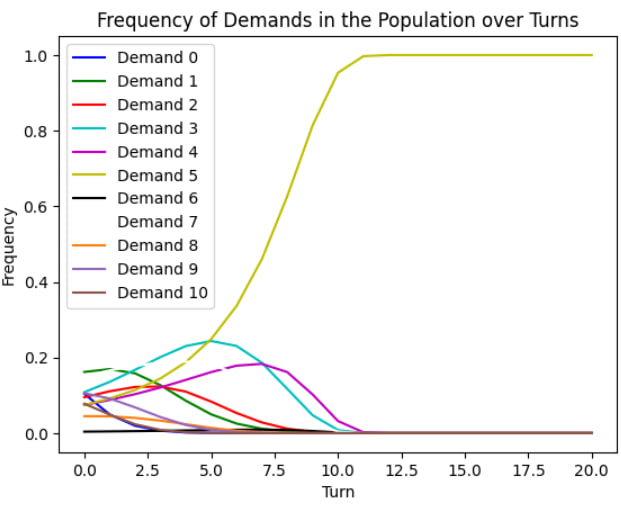
\includegraphics{16}
\end{center}

\begin{center}
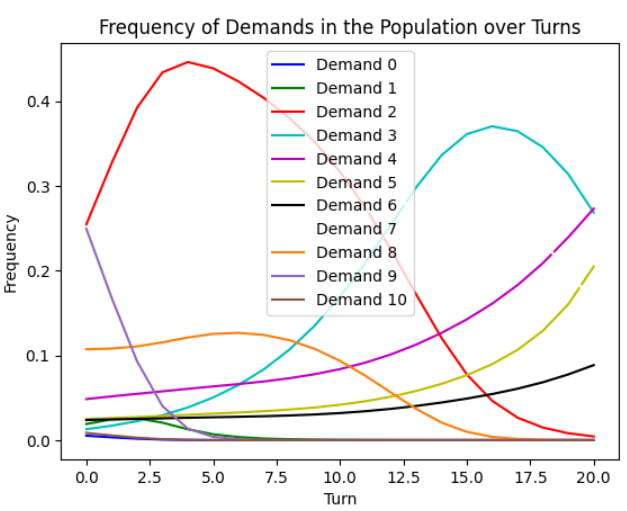
\includegraphics{17}
\end{center}

\begin{center}
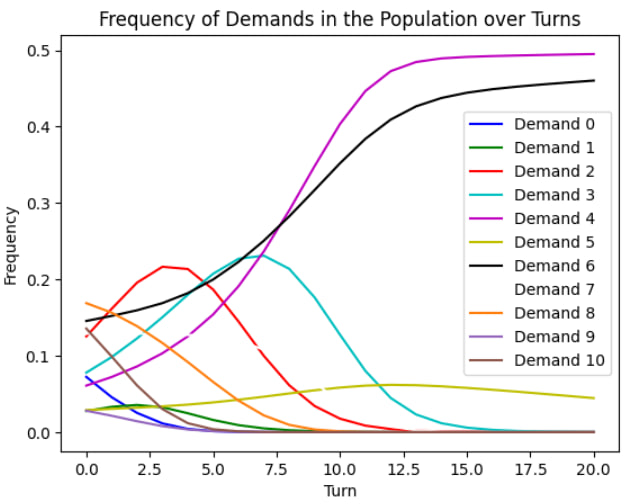
\includegraphics{18}
\end{center}

\begin{center}
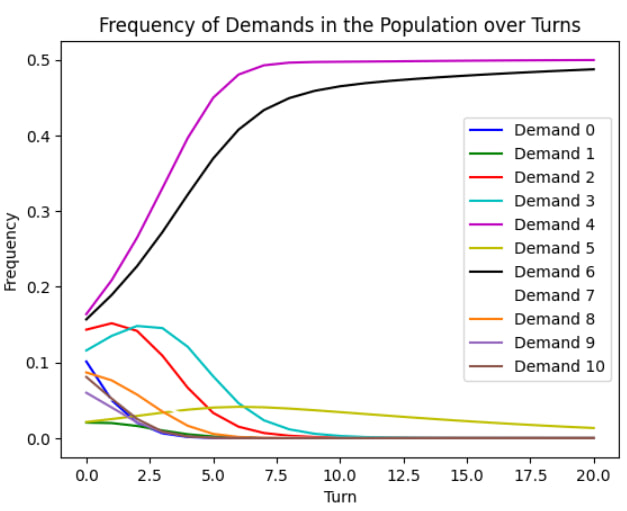
\includegraphics{19}
\end{center}

\begin{center}
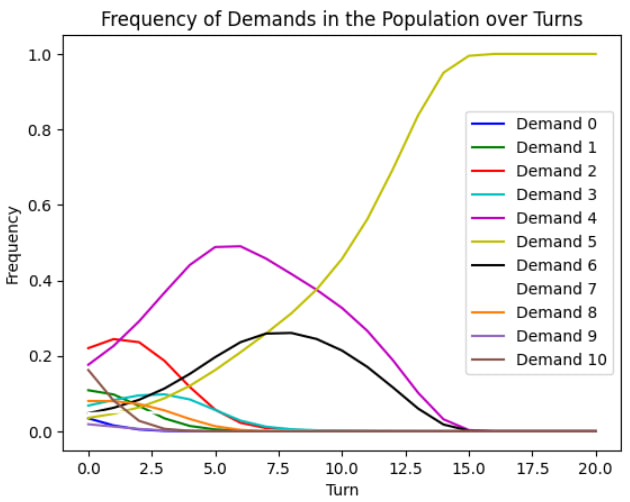
\includegraphics{20}
\end{center}

یک نکته مهم که باید به آن توجه کنیم، تأمین نیازهای یکدیگر توسط اعضای جامعه است. به این معنی که استراتژی‌ها باید به یکدیگر متمم باشند و در عین حال باید توزیع پاداش به صورت منصفانه‌ای انجام شود. در استراتژی ۵، این دو شرط همواره برقرار است و در نتیجه، این استراتژی همیشه به عنوان استراتژی پایدار در هر شرایطی عمل می‌کند. احتمالاً ترکیبی از استراتژی‌های ۴ و ۶ می‌تواند نیازهای جامعه را برآورده کند، اما به طور کامل منصفانه نخواهد بود.

بنابراین، نتیجه‌گیری می‌شود که پس از تعدادی دور، در نهایت به استراتژی ۵ می‌رسیم (مگر اینکه در ابتدای بازی این استراتژی از بین برود) و این استراتژی یک تعادل پایدار برای بازی خواهد بود. این تعادل نشان دهنده توازنی است که به دست می‌آید و بازیکنان در آن به صورت پایدار بازی می‌کنند.
